\frame
{
	\frametitle{Acquisition d'un \'equipement}
	\begin{enumerate}
		\item Avant achat, soumission d'un appel d'offres
		\begin{itemize}
			\item<2-> D\'efinition d'une liste de use cases.

                Exemple: les images brutes export\'ees pourront \^etre r\'eutilis\'ees \emph{a posteriori}.
			\item<3-> R\'edaction du cahier des charges en incluant DICOM et IHE.
			\begin{itemize}
				\item<3-> Pr\'eciser les exigences en termes DICOM et IHE
				
				$\rightarrow$ gr\^ace aux comp\'etences internes,
				
				$\rightarrow$ ou en faisant appel \`a une expertise externe.
				\item<4-> Exiger des documents de conformit\'e DICOM (DICOM Conformance Statement, IHE International Conformity Assessment, r\'esultats Connectathon, etc.).
			\end{itemize}
		\end{itemize}
		\item<5-> Acceptation protocol\'ee
		\begin{itemize}
			\item<6-> V\'erification de la conformit\'e aux profils demand\'es.
			\item<7-> Tests et qualification sur la base des uses cases impliquant
			\begin{itemize}
				\item<8-> le fournisseur,
				\item<9-> le biom\'edical,
				\item<10-> le service informatique,
				\item<11-> les utilisateurs.
			\end{itemize}
		\end{itemize}
	\end{enumerate}
}

\frame
{
	\frametitle{Services \`a demander}
	\begin{center}
		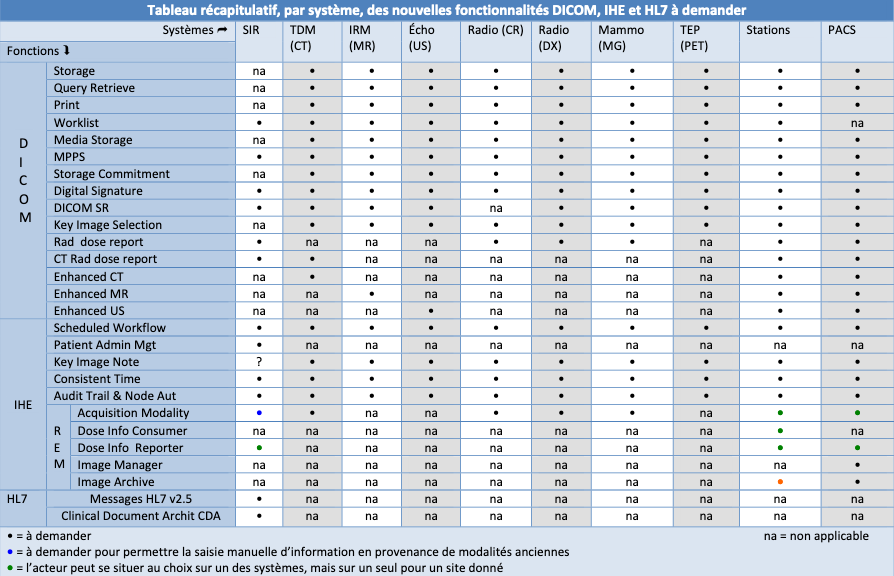
\includegraphics[width=\linewidth]{../figures/tableau-services.png}
	\end{center}
}